\newpage

\section{Analisi dei rischi}

Al fine di ridurre al minimo i possibili ritardi sulla pianificazione e migliorare la qualità del progetto, vengono di seguito analizzati i rischi che potrebbero insorgere nel corso dello sviluppo.\\

È possibile prendere visione dei rischi che si sono effettivamente riscontrati durante i periodi di progetto nell'\hyperref[RiscontroRischi]{Appendice A}.\\
Di seguito la tabella con i rischi individuati, divisi a seconda del livello di appartenenza:

\subsection{Livello tecnologico}
\begin{table}[h!]
	\centerline{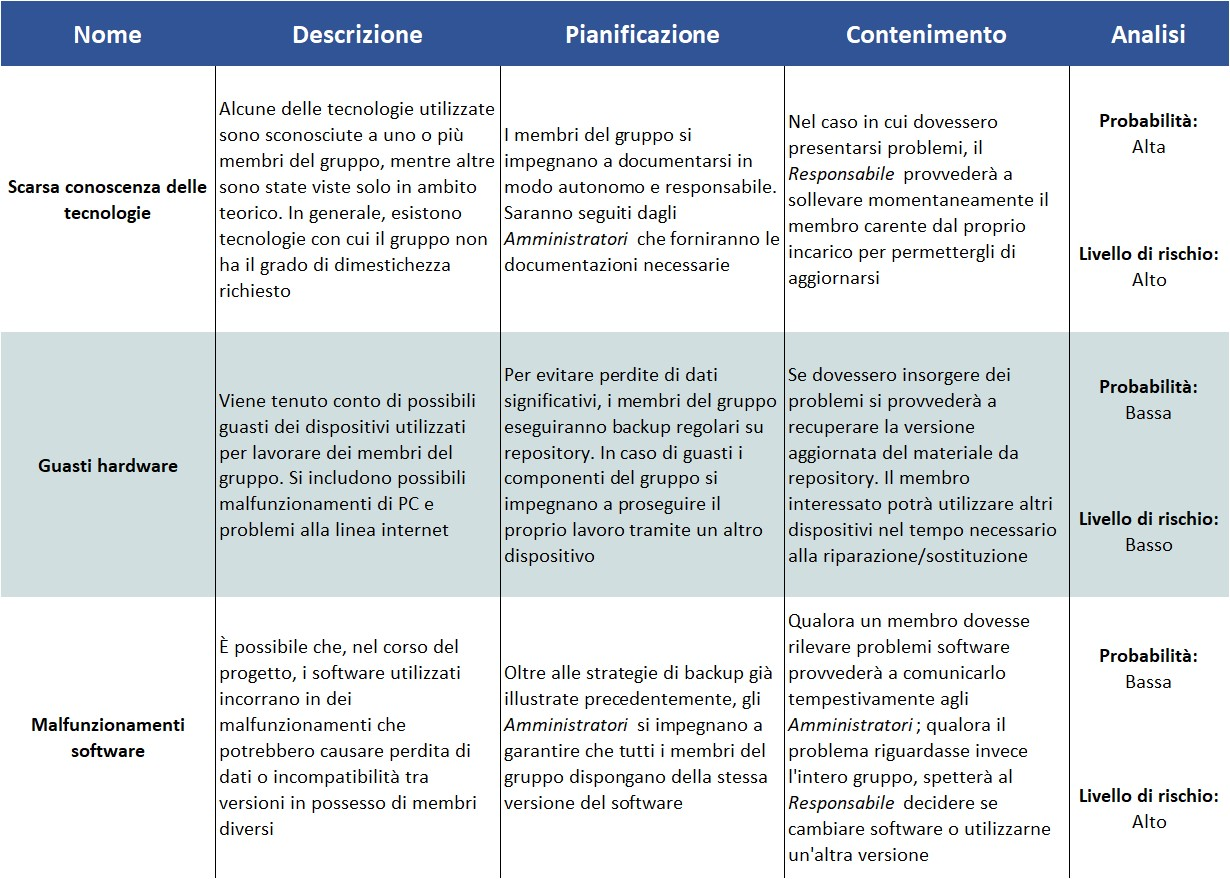
\includegraphics[scale=0.55]{img/Rischi/LivelloTecnologico.jpg}}
	\caption{Tabella dei rischi: Livello Tecnologico}
\end{table}
\clearpage

\subsection{Livello personale}
\begin{table}[h!]
	\centerline{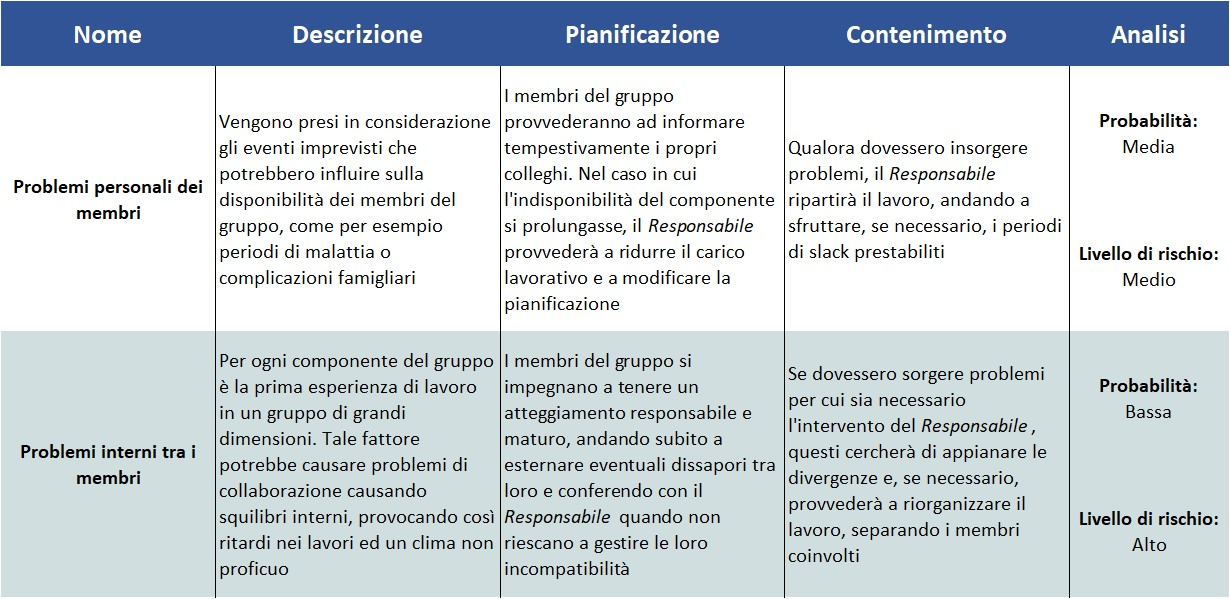
\includegraphics[scale=0.55]{img/Rischi/LivelloPersonale.jpg}}
	\caption{Tabella dei rischi: Livello Personale}
\end{table}
\clearpage

\subsection{Livello organizzativo}
\begin{table}[h!]
	\centerline{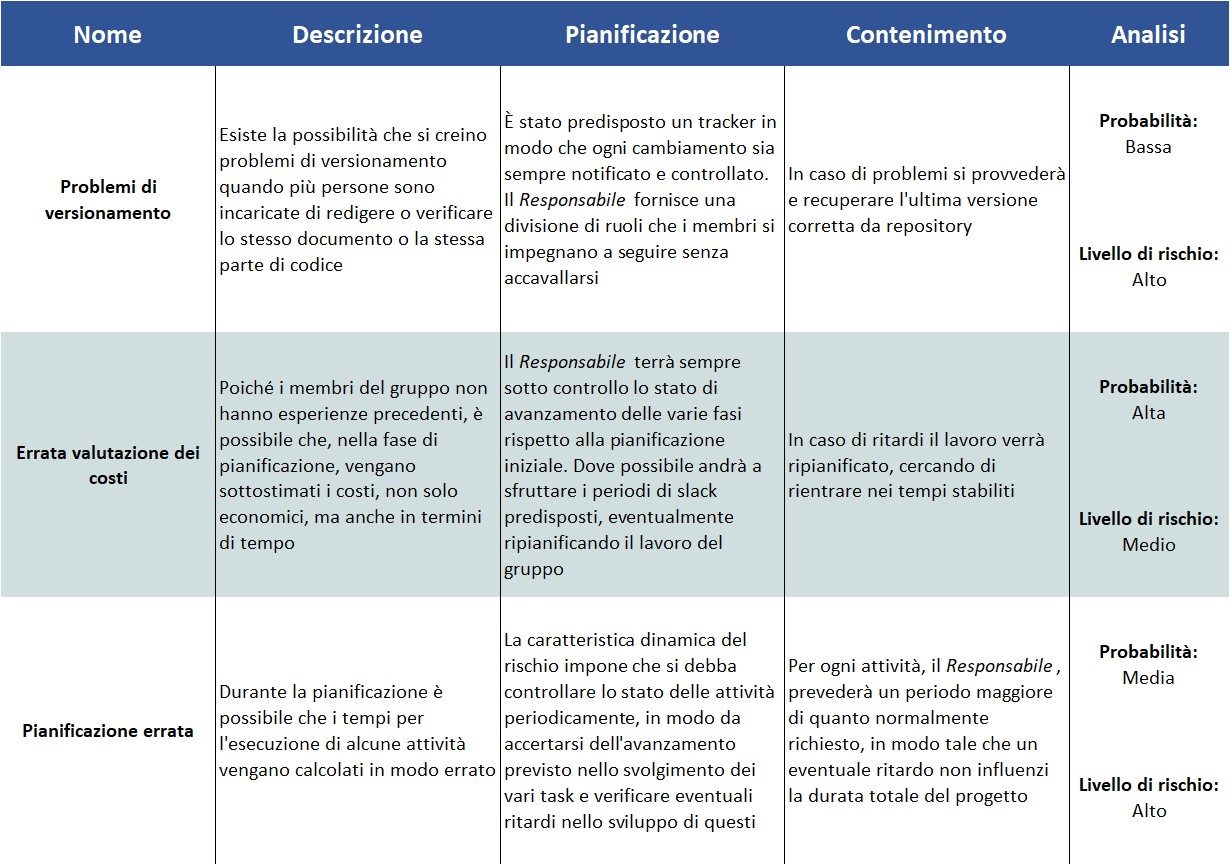
\includegraphics[scale=0.55]{img/Rischi/LivelloOrganizzativo.jpg}}
	\caption{Tabella dei rischi: Livello Organizzativo}
\end{table}
\clearpage

\subsection{Strumenti}
\begin{table}[h!]
	\centerline{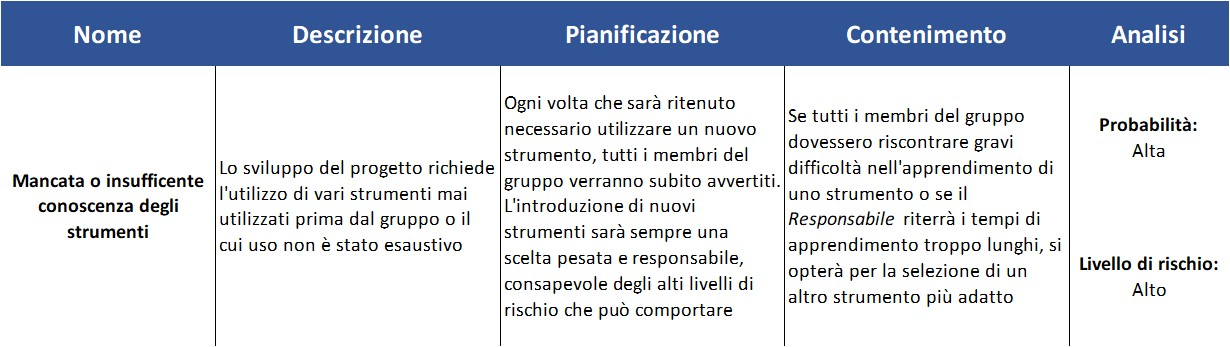
\includegraphics[scale=0.55]{img/Rischi/Strumenti.jpg}}
	\caption{Tabella dei rischi: Strumenti}
\end{table}

\subsection{Requisiti}
\begin{table}[h!]
	\centerline{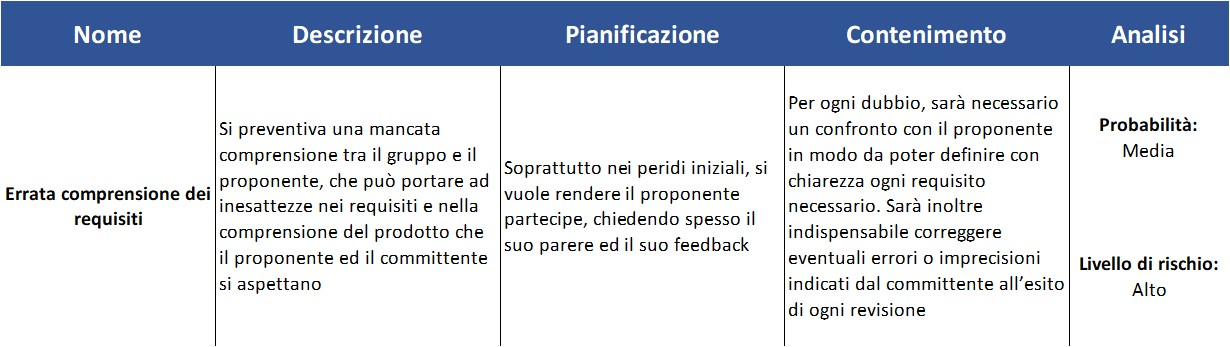
\includegraphics[scale=0.55]{img/Rischi/Requisiti.jpg}}
	\caption{Tabella dei rischi: Requisiti}
\end{table}
\clearpage